\documentclass{article}
\usepackage[italian]{babel}
\usepackage{microtype}
\usepackage[utf8]{inputenc}
\usepackage{hyperref}
\usepackage[italian]{cleveref}
\usepackage[sort, round]{natbib}
\usepackage{graphicx}
\usepackage[margin=2cm]{geometry}
\usepackage[table,xcdraw]{xcolor}
\usepackage{listings}
\usepackage{parskip}

\definecolor{codegreen}{rgb}{0,0.6,0}
\definecolor{codegray}{rgb}{0.5,0.5,0.5}
\definecolor{codepurple}{rgb}{0.58,0,0.82}
\definecolor{backcolour}{rgb}{0.95,0.95,0.92}

\lstdefinestyle{mystyle}{
    backgroundcolor=\color{backcolour},
    commentstyle=\color{codegreen},
    keywordstyle=\color{magenta},
    numberstyle=\tiny\color{codegray},
    stringstyle=\color{codepurple},
    basicstyle=\ttfamily\footnotesize,
    breakatwhitespace=false,
    breaklines=true,
    captionpos=b,
    keepspaces=true,
    numbers=left,
    numbersep=5pt,
    showspaces=false,
    showstringspaces=false,
    showtabs=false,
    tabsize=2
}

\lstset{style=mystyle}

\title{Q-learning su FPGA \\ Progetto d'esame per il corso di Sistemi Digitali M}
\date{\today}
\author{Davide Ragazzini \and Kevin Michael Frick}

\begin{document}
\maketitle

\section{Introduzione}
Il \emph{reinforcement learning} è una branca dell'apprendimento macchina orientato allo sviluppo di algoritmi in grado di massimizzare la \emph{funzione di reward} totale in un \emph{processo decisionale Markoviano}, ovvero un \emph{ambiente} che espone uno \emph{stato} e delle \emph{azioni}. 

Questi algoritmi tentano di stimare una funzione $q(s, a)$ che restituisce la massima reward ottenibile scegliendo l'azione $a$ quando l'ambiente è nello stato $s$.
Questa stima viene poi utilizzata per definire una \emph{policy} $\pi(s, a)$ che determina la probabilità di scegliere l'azione $a$ quando il sistema è nello stato $s$. 
Si opera una distinzione tra algoritmi \emph{on-policy}, i quali mantengono una sola policy che viene continuamente aggiornata e utilizzata per scegliere l'azione migliore, e algoritmi \emph{off-policy} che invece mantengono una stima della policy ottimale che viene aggiornata basandosi su dati relativi a esperienze precedenti che vengono elaborati. 
Gli algoritmi più recenti si servono di reti neurali, che si possono dimostrare essere in grado di approssimare funzioni qualunque, ma esistono algoritmi detti \emph{classici} come Q-learning \citep{watkins_learning_1989}. 

Q-learning è un algoritmo on-policy che si serve di una matrice stato-azione $Q$ (da cui il nome) la cui cella corrispondente alla riga $s$ e colonna $a$ contiene una stima della reward totale per lo stato $s$ l'azione $a$. 
A ogni periodo $t$ l'agente seleziona un'azione $a_t$, osserva la reward $r_t$ e transiziona allo stato $s_{t + 1}$ funzione dello stato corrente $s_t$ e dell'azione $a_t$. 
È evidente come questo algoritmo possa essere applicato solamente a casi in cui lo spazio degli stati e quello delle azioni sono discreti. 
In presenza di uno spazio degli stati continuo, come nel task scelto per questo progetto, è necessario progettare un modulo che si occupi di operare una discretizzazione degli stati. 

A ogni iterazione dell'algoritmo la matrice $Q$ viene aggiornata secondo la seguente espressione

$$
Q'(s_t, a_t) \leftarrow Q(s_t, a_t) + \alpha (r_t + \gamma \max_a Q(s_{t+1}, a) - Q(s_t, a))
$$

dove $\gamma \in [0, 1)$ è detto \emph{discount factor} e $\alpha$ è detta \emph{learning rate} o \emph{passo}.
Questi metaparametri hanno valori ottimali che variano a seconda del task a cui viene applicato l'algoritmo. 
Le metodologie di reinforcement learning, difatti, hanno applicazioni in svariati contesti, dal controllo di sistemi complessi \citep{hu_voronoi-based_2020} alla simulazione di dinamiche di mercato \citep{calvano_artificial_2020}.
Esistono inoltre task ``didattici'' standardizzati il cui scopo è valutare le prestazioni delle varie implementazioni di questo tipo di algoritmi.

Il discount factor è utilizzato per dare un valore maggiore alle reward ricevute all'inizio, esprimendo il concetto di ``buona partenza''. 
Se $\gamma < 1$ le reward convergono a 0 all'aumentare del numero di periodi.
Si può dimostrare che ciò assicura che la convergenza dell'algoritmo. 

Il passo determina la velocità di variazione delle stime della funzione $q(\cdot)$ e di conseguenza la velocità di convergenza. 
Impostare un passo troppo alto può portare a cicli e mancata convergenza, mentre  valori troppo bassi rallentano drammaticamente la velocità di convergenza dell'algoritmo. 
Il passo non è necessariamente fisso. 
Al contrario, spesso si utilizza un passo \emph{adattivo}, che cambia sulla base dei risultati ottenuti (ad esempio aumentando se non si verifica un aumento della reward media per molti periodi), oppure un passo \emph{calante} secondo una formula data. 

Il reinforcement learning differisce dall'apprendimento supervisionato perché non corregge esplicitamente le azioni non ottime basandosi su "esempi di correttezza" bensì esplora lo spazio delle azioni e delle reward in base a una politica data. 
Questa politica è solitamente \emph{greedy}, se sceglie sempre l'azione migliore trovata fino a quel momento (scelta detta \emph{exploitation}),  o \emph{$\epsilon$-greedy}, se invece a ogni periodo vi è una probabilità $\epsilon \in (0, 1)$ di scegliere casualmente un'azione per ``vedere cosa succede'' (scelta detta \emph{exploration}). 
Come per il passo, i valori di $\epsilon$ influiscono sulla velocità di convergenza: valori troppo alti significano che la conoscenza acquisita non viene sfruttatta efficientemente, mentre valori troppo bassi portano l'algoritmo a convergere su valori di reward medie più basse.
Sempre come nel caso del passo, $\epsilon$ è solitamente un parametro adattivo o calante. 

\section{Implementazione}
L'algoritmo è stato implementato servendosi di Vitis HLS, Vivado e Vitis nella versione 2020.2. 
I test sono stati eseguiti su una ZedBoard, una development board per la FPGA Zynq-7000 All Programmable SoC XC7Z020-CLG484-1, con periodo di clock impostato a $T = 10 \textrm{ns}$.
È stato scelto come caso di test il task \emph{CartPole}.
Questo task prevede l'apprendimento di una policy che permetta di bilanciare un bastone in equilibrio su un carrello che può essere spostato a destra e a sinistra.
Si tratta cioè di simulare un sistema fisico che abbia la dinamica di un \emph{pendolo invertito}. 

Le variabili di stato di questo task sono:

\begin{itemize}
\item $x$, la posizione del carrello
\item $\dot{x}$, la velocità del carrello
\item $\theta$, l'angolo formato dall'asta del pendolo e dall'asse orizzontale
\item $\dot{\theta}$, la velocità angolare dell'estremità superiore del pendolo
\end{itemize}

Le azioni disponibili sono solo due: spostare il carrello di un intervallo $\delta x$ a destra o a sinistra, ovvero $A = \{x \leftarrow x + \delta x, x \leftarrow x - \delta x\}$. 

Si è scelto di impostare il discount factor a $\gamma = 0.999$ e una learning rate calante secondo la formula $\alpha = \log_{10}\frac{t + 1}{25}$, seguendo la letteratura concernente il task scelto \citep{sutton_reinforcement_2018}.
Il parametro $\epsilon$ è anch'esso calante secondo la formula $\epsilon = 0.9 + (0.9 - 0.05) e^{-\frac{t}{200}}$.

Il codice HLS, lo schema a blocchi per Vivado e il codice per la PS sono rilasciati sotto licenza GPLv3 all'indirizzo \url{https://github.com/kmfrick/HLS_QLearning}.
\subsection{Vitis HLS}
Il cuore del progetto è una IP che implementa Q-learning, realizzata nel linguaggio C++ e tradotta in VHDL mediante il software Vitis HLS. 

La top-function dell'IP generata è \texttt{learn()}, che riceve in input un \texttt{hls::stream} di numeri casuali a 32 bit, utilizzati per decidere tra exploration ed exploitation con probabilità $\epsilon$ di exploration e scegliere casualmente un'azione in caso di exploration. 
Si è scelto di disaccoppiare la generazione di numeri casuali dalla top-function di apprendimento, inserendo una direttiva che richieda a Vitis HLS di tradurre questo argomento in una porta AXI-Stream sulla IP generata. 
Gli altri argomenti della top-function sono la porta di uscita \texttt{running}, che verrà poi collegata ai LED della ZedBoard per fornire informazioni sullo stato dell'IP, la porta di ingresso \texttt{id} contenente un identificatore dell'agente, cablato a 0, e le due porte di I/O \texttt{failures} e \texttt{q\_table} che verrano mappate alla DRAM del PS mediante il protocollo AXI4 Lite, nel bundle \texttt{shared}.
Il valore restituito dalla top function è comunicato al PS mediante il protocollo AXI4 Lite, nel bundle \texttt{return}.
L'azione scelta e lo stato attuale sono passati alla \texttt{get\_state()} che restituisce lo stato risultante. 
Il codice della \texttt{get\_state()} è il seguente:

\begin{lstlisting}[language=C++]
int get_state() {

	printf("Hello, World!");
	return 0;
}
\end{lstlisting}
Lo spazio degli stati è continuo con dimensione 4, ma viene mappato a un insieme limitato di 162 possibili stati, le righe della matrice $Q$, mediante la funzione \texttt{discretize()}. 

Il codice della \texttt{discretize()} è il seguente:
\begin{lstlisting}[language=C++]
int discretize(float x, float x_dot, float theta, float theta_dot) {
        int box = 0;

        if (x < -X_BOUND || x > X_BOUND || theta < -twelve_degrees
                        || theta > twelve_degrees)
                return (-1); // to signal failure

        if (x < -0.8f)
                box = 0;
        else if (x < 0.8f)
                box = 1;
        else
                box = 2;

        if (x_dot < -0.5f)
                // noop
                ;
        else if (x_dot < 0.5f)
                box += 3;
        else
                box += 6;

        if (theta < -six_degrees)
                // noop
                ;
        else if (theta < -one_degree)
                box += 9;
        else if (theta < 0)
                box += 18;
        else if (theta < one_degree)
                box += 27;
        else if (theta < six_degrees)
                box += 36;
        else
                box += 45;

        if (theta_dot < -fifty_degrees)
                ;
        else if (theta_dot < fifty_degrees)
                box += 54;
        else
                box += 108;

        return (box);
}
\end{lstlisting}

Fattorizzando la funzione di stato futuro e la discretizzazione delle azioni e avendo cura di definire in maniera appropriata costanti che rappresentino la dimensione dello spazio degli stati e delle azioni, la top-function può rimanere inalterata al variare dei task ed è possibile adattare l'IP a un nuovo task scrivendo solamente queste due funzioni. 

La convergenza è definita come l'apprendimento di una policy in grado di bilanciare il pendolo per almeno 195 periodi in media mobile sulle ultime 50 epoche. 

Nella tabella \labelcref{table:synthesis} vengono riportati i risultati della sintesi VHDL della IP in termini di utilizzo di risorse e periodo di clock. 

\begin{table}[h!]

\centering

\begin{tabular}{|c|c|}
\hline
 &VHDL \\
 \hline
SLICE &0 \\
 \hline
LUT &5036 \\
 \hline
FF &4566 \\
 \hline
DSP &19 \\
 \hline
BRAM &6 \\
 \hline
SRL &138 \\
 \hline

\end{tabular}

\vspace{1em}

\begin{tabular}{|c|c|}
\hline 
 &VHDL \\
 \hline 
CP required &10.000 \\
 \hline 
CP achieved post-synthesis &8.276 \\
 \hline 
\end{tabular}
\caption{Report di sintesi di Vitis HLS}
\label{table:synthesis}

\end{table}
\subsection{Vivado}
Si è scelto di usare una IP open source \citep{fedorko_wfedorkomersenne-twister-hls_2018} che implementa l'algoritmo Mersenne Twister per generare numeri casuali. 

Lo schema a blocchi definito su Vivado è rappresentato in fig. \labelcref{fig:bd}.
\begin{figure}[h!]

\centering


\includegraphics[width=\textwidth]{bd.png}
\caption{Schema a blocchi del sistema progettato}
\label{fig:bd}
\end{figure}

Una AXI Interconnect permette di collegare i blocchi che accedono alla memoria e mappare le variabili di ingresso e uscita sulla DRAM del PS. 

\subsection{Vitis}
È stata sviluppata un'applicazione bare-metal su PS per avviare l'IP, gestirne i dati in input e automatizzare i test prestazionali. 
Si è scelto di testare le differenze che si vedono inizializzando la matrice $Q$ a 0, inizializzandola con valori casuali tra 0 e 1  e inizializzandola con valori casuali tra 4 e 5 (optimistic initial values). 

\subsection{Stima dell'occupazione della memoria}
\subsection{Problemi di implementazione}
Durante lo sviluppo di questa soluzione, è sorta la questione di come gestire l'input e l'output delle variabili, in modo da realizzare una soluzione integrabile in modo semplice in pipeline già esistenti. 
Data la possibilità di interagire con il PS tramite UART, si è scelto di sviluppare un'applicazione bare-metal su PS. 

Un altro punto aperto è quello relativo alla massima dimensione della matrice stato-azione che possa essere memorizzata. 
Un singolo elemento di una matrice $Q$ è un numero in virgola mobile a 32 bit (4 byte).
La ZedBoard utilizzata per la valutazione dispone di 512 MiB di DRAM.
Senza considerare l'\emph{overhead} introdotto dal modulo di generazione di numeri casuali, sarebbe quindi possibile sulla carta memorizzare una matrice $Q$ con più di 100 milioni di elementi. 
La scelta exploration/exploitation e dell'azione in caso di exploration richiede la generazione di numeri casuali \citep{sutton_reinforcement_2018}.
La libreria standard C implementa un \emph{generatore congruenziale lineare} che però mal si presta a essere sintetizzato su FPGA a causa dell'alto consumo di risorse fisiche. 
Per questo motivo si è scelto di usare una IP open source \citep{fedorko_wfedorkomersenne-twister-hls_2018} che implementa l'algoritmo Mersenne Twister per generare numeri casuali.

In generale, il tema dell'efficienza in termini di risorse fisiche è spesso ritornato e sono stati presi accorgimenti per minimizzare la quantità di LUT usate: le \emph{learning rate} e i parametri $\epsilon$ corrispondente a ogni epoca, ad esempio, sono stati precalcolati e inseriti in un array statico. 

In preparazione della parallelizzazione ci si è posti il problema di come condividere la memoria tra più copie della stessa IP. 
L'uso di blocchi di BRAM non è appropriato. 
L'alta velocità di accesso a questo tipo di memoria, infatti, non è necessaria per questo tipo di applicazioni, nel quale il numero di periodi è relativamente ridotto e il parametro rilevante per la valutazione di un'implementazione è il numero di periodi necessari per la convergenza.
Per questo motivo si è optato per l'uso della DRAM.

\section{Prestazioni}
L'algoritmo è stato testato passando in input 1000 \emph{seed} diversi per il generatore di numeri casuali che determina exploration/exploitation.
I risultati ottenuti in media tra i 1000 seed sono riportati nella tabella \labelcref{table:perf} e visualizzati nella fig. \labelcref{fig:perf}.

\begin{figure}[h!]

\centering


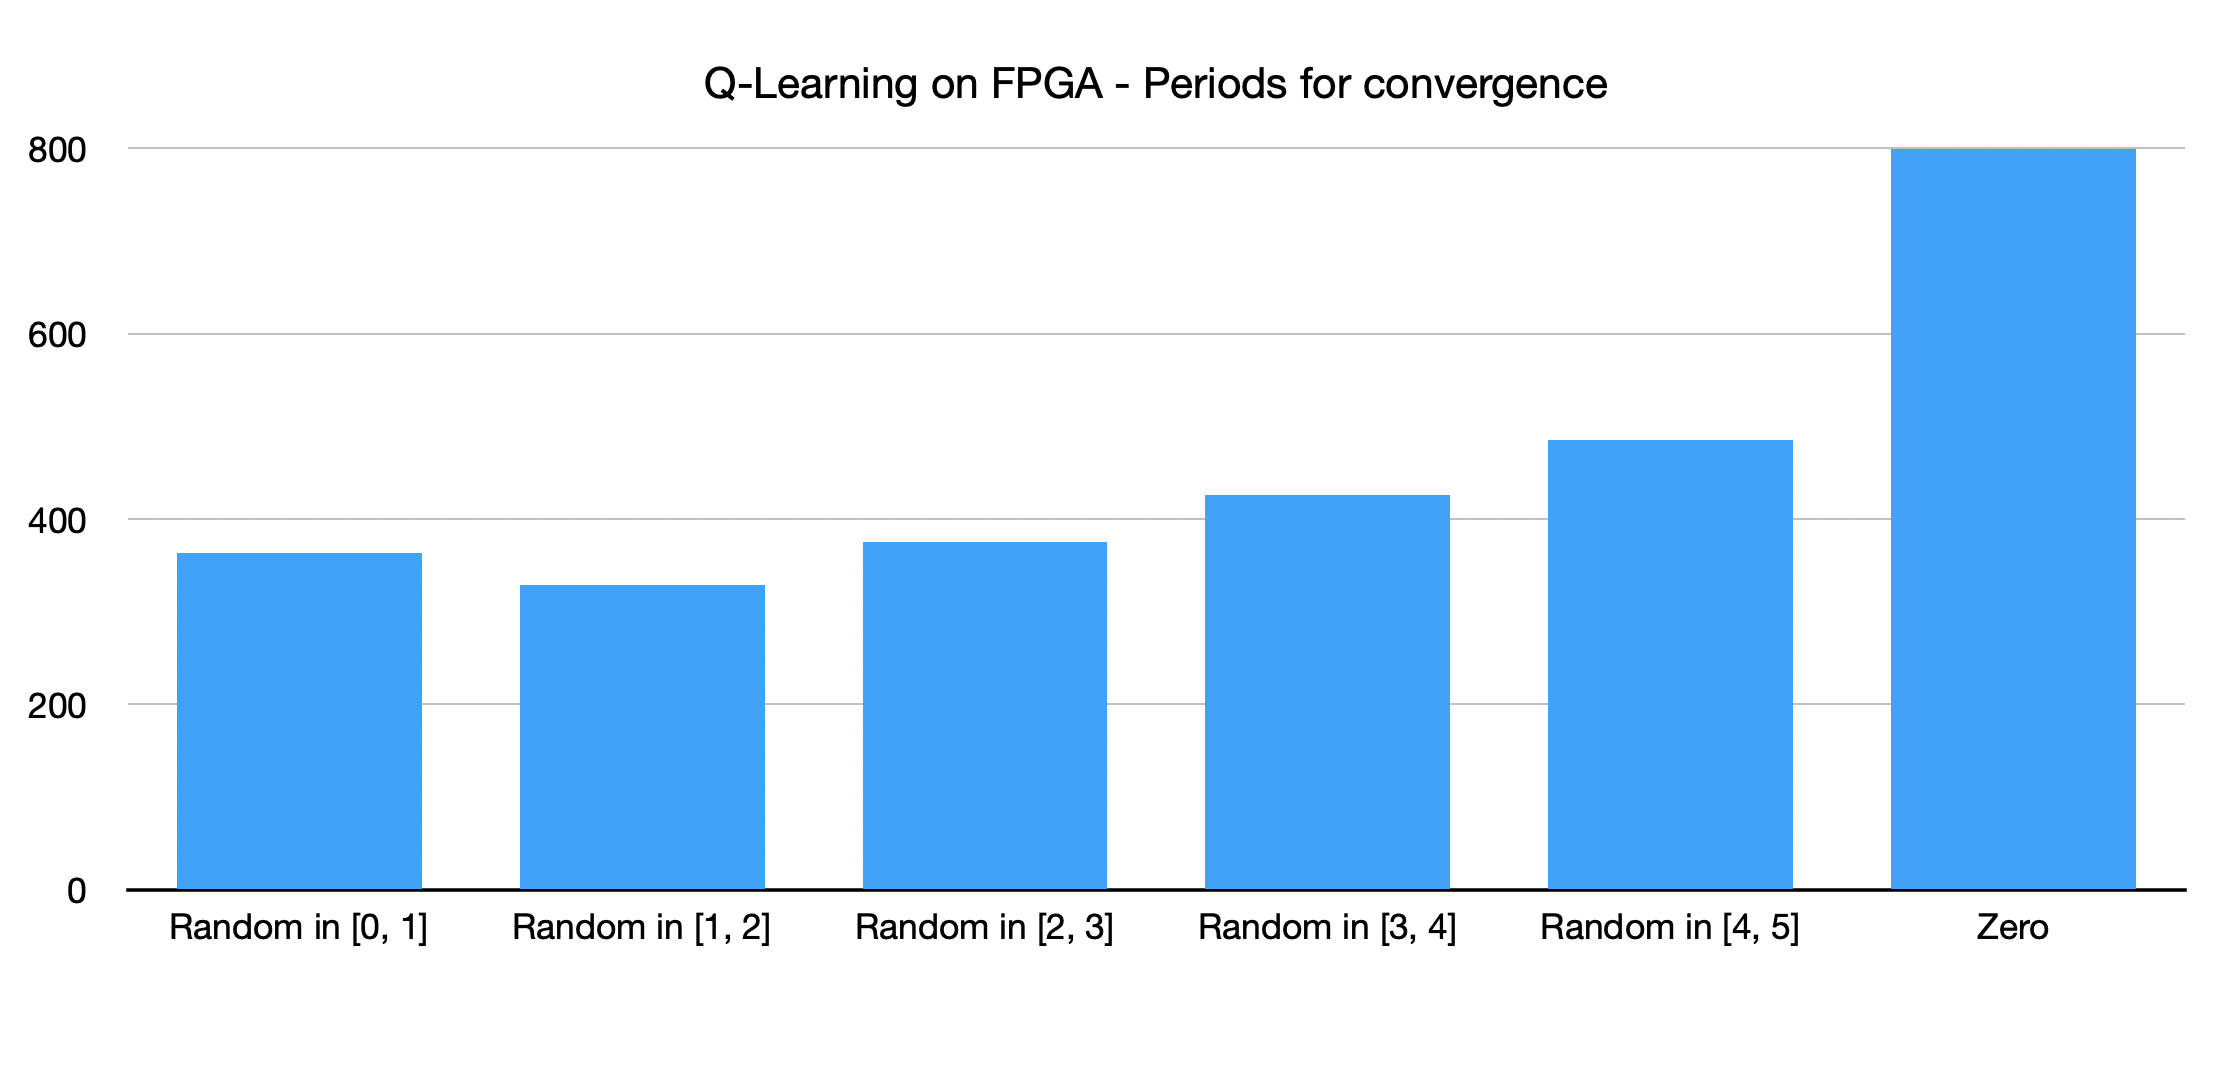
\includegraphics[width=0.5\textwidth]{perf.png}
\caption{Prestazioni sperimentali medie}
\label{fig:perf}
\end{figure}

\begin{table}[h!]

\centering


\begin{tabular}{|
	>{\columncolor[HTML]{EFEFEF}}l |l|}
	\hline
	& \cellcolor[HTML]{EFEFEF}\textbf{Periodi per la convergenza} \\ \hline
	\textbf{Inizializzazione casuale}             &                                                                 \\ \hline
	\textbf{Inizializzazione casuale ottimistica} &                                                                 \\ \hline
	\textbf{Inizializzazione a 0}                 &                                                                 \\ \hline
	\textbf{}                                     &                                                                 \\ \hline
	\end{tabular}
	\caption{Prestazioni sperimentali medie}
	\label{table:perf}
	\end{table}

	Come è noto e ampiamente discusso in letteratura \citep{sutton_reinforcement_2018}, l'inizializzazione a valori casuali ottimistici migliora la velocità di convergenza. 
	La velocità media di convergenza è comunque minore di quella ottenuta da altre implementazioni dell'algoritmo, probabilmente a causa degli errori di arrotondamento portati dall'utilizzo di variabili in virgola mobile a 32 bit, reso necessario dalla ridotta disponibilità di memoria su FPGA.
	\section{Evoluzioni future}
	Il codice HLS è stato impostato in modo da permettere l'implementazione di apprendimento multiagente \citep{kretchmar_parallel_2002} mediante la condivisione degli array \texttt{failures} e \texttt{q} tra più moduli uguali nella PL.
	L'implementazione e il testing di questo tipo di apprendimento saranno oggetto dell'attività progettuale di Sistemi Digitali M.
	\bibliographystyle{plainnat}
	\bibliography{main}
	\end{document}

